 
\section{``Proofs'' section (To Be Incorporated into Section \ref{sec:analytics})}

\subsection{Proof that all density one packings are such that $N$ is either a perfect square or expressible as the sum of two squares}

\begin{enumerate}
\item For a density one packing, all squares must be oriented in the same way, and must touch one another [share a common edge?].

JM:  For a density one packing every square must have at least four other squares that contact it along a finite segment length and thus all squares must be oriented in the same direction.

\item For any three squares that touch one another and are oriented the same way, two of those squares must be in a row. (See Figure \ref{fig:aligned}).

\item Therefore, all density one packings are arranged in rows.

\item If squares on the torus are arranged in rows, the periodicity requirement of the toroidal packing ensures that the number of squares $N$ in the packing may be computed as $N=a^2+b^2$, via the Pythagorean theorem (Figure \ref{fig:pythagoras}).

\item Therefore, all density one packings are such that $N$ is either a perfect squares or expressible as a sum of two squares.
\end{enumerate}


\subsection{Entropy of packings with density $=1$ [$N=( \sqrt N)^2$ or $N=a^2+b^2$]}

\begin{enumerate}
\item For density one packings, all squares must be arranged in rows (see above).
\item For some density one packings, it may be possible to shift rows relative to one another, increasing the entropy of these packings.
\item The entropy of such packings will therefore be proportional to the number of rows that can be shifted independently of one another.
\item From Figure \ref{fig:Bezout}, it can be seen that the number of rows that can be shifted independently is proportional to the smallest integer that can be written in the form $a n_2 + b n_4$, where $n_2$ and $n_4$ are defined as in Section \ref{sec:analytics}, and $a$ and $b$ are integers.
\item Bezout's Lemma [REF] states that this integer linear combination cannot be smaller than $d$, the greatest common divsor of $n_2$ and $n_4$. 

JM: "cannot be smaller than" -> "can be made equal to but not smaller than"

\item There are therefore $d$ rows that can be shifted independently of one anaother; thus the entropy of density one packings is proportional to $d$.
\end{enumerate}


\subsection{Proof that the thermodynamic limit allows for any arbitrary orientation of the square lattice on the torus, so that orientational symmetry is not broken.}


\begin{enumerate}
\item $N=a^2+b^2$ solutions select an orientation of the square lattice on the torus via the ratio $a/b$.

JM:  If $N=N_1^2 + n_2^2$ the packing selects and orientation of the squares that is oriented at an angle $\tan^{-1}(n_2/n_1)$ relative to the torus lattice vectors.

Use $n_1$ and $n_2$ rather than $a$ and $b$.

\item The thermodynamic limit can be reached via an infinite sequence of $N=a^2+b^2$ solutions such that $\frac{a}{b}$ equals some constant $r$, which picks out a particular orientation of the square lattice as $N \rightarrow \infty $. 

JM: If $r$ is irrational the ratio approaches $r$ but does not equal $r$.

\item Therefore any particular orientation of the square lattice on the torus may be selected by reaching the thermodynamic limit via the appropriately chosen sequence of $N$, and rotational symmetry is not broken.

JM: The thermodynamic limit must be taken as a {\em subsequence} of the integers.
\end{enumerate}


\begin{figure}[H]
\label{fig:aligned}
\scalebox{.3}{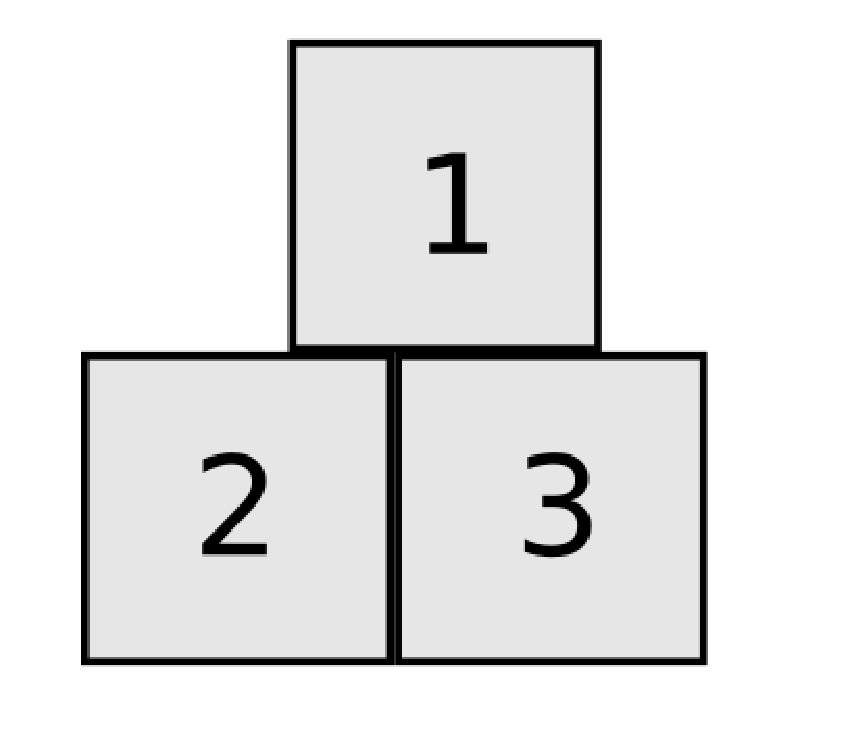
\includegraphics{figures/alignedBlocks.pdf}}
\caption{}
\end{figure}

\begin{figure}[H]
\label{fig:pythagoras}
\scalebox{.3}{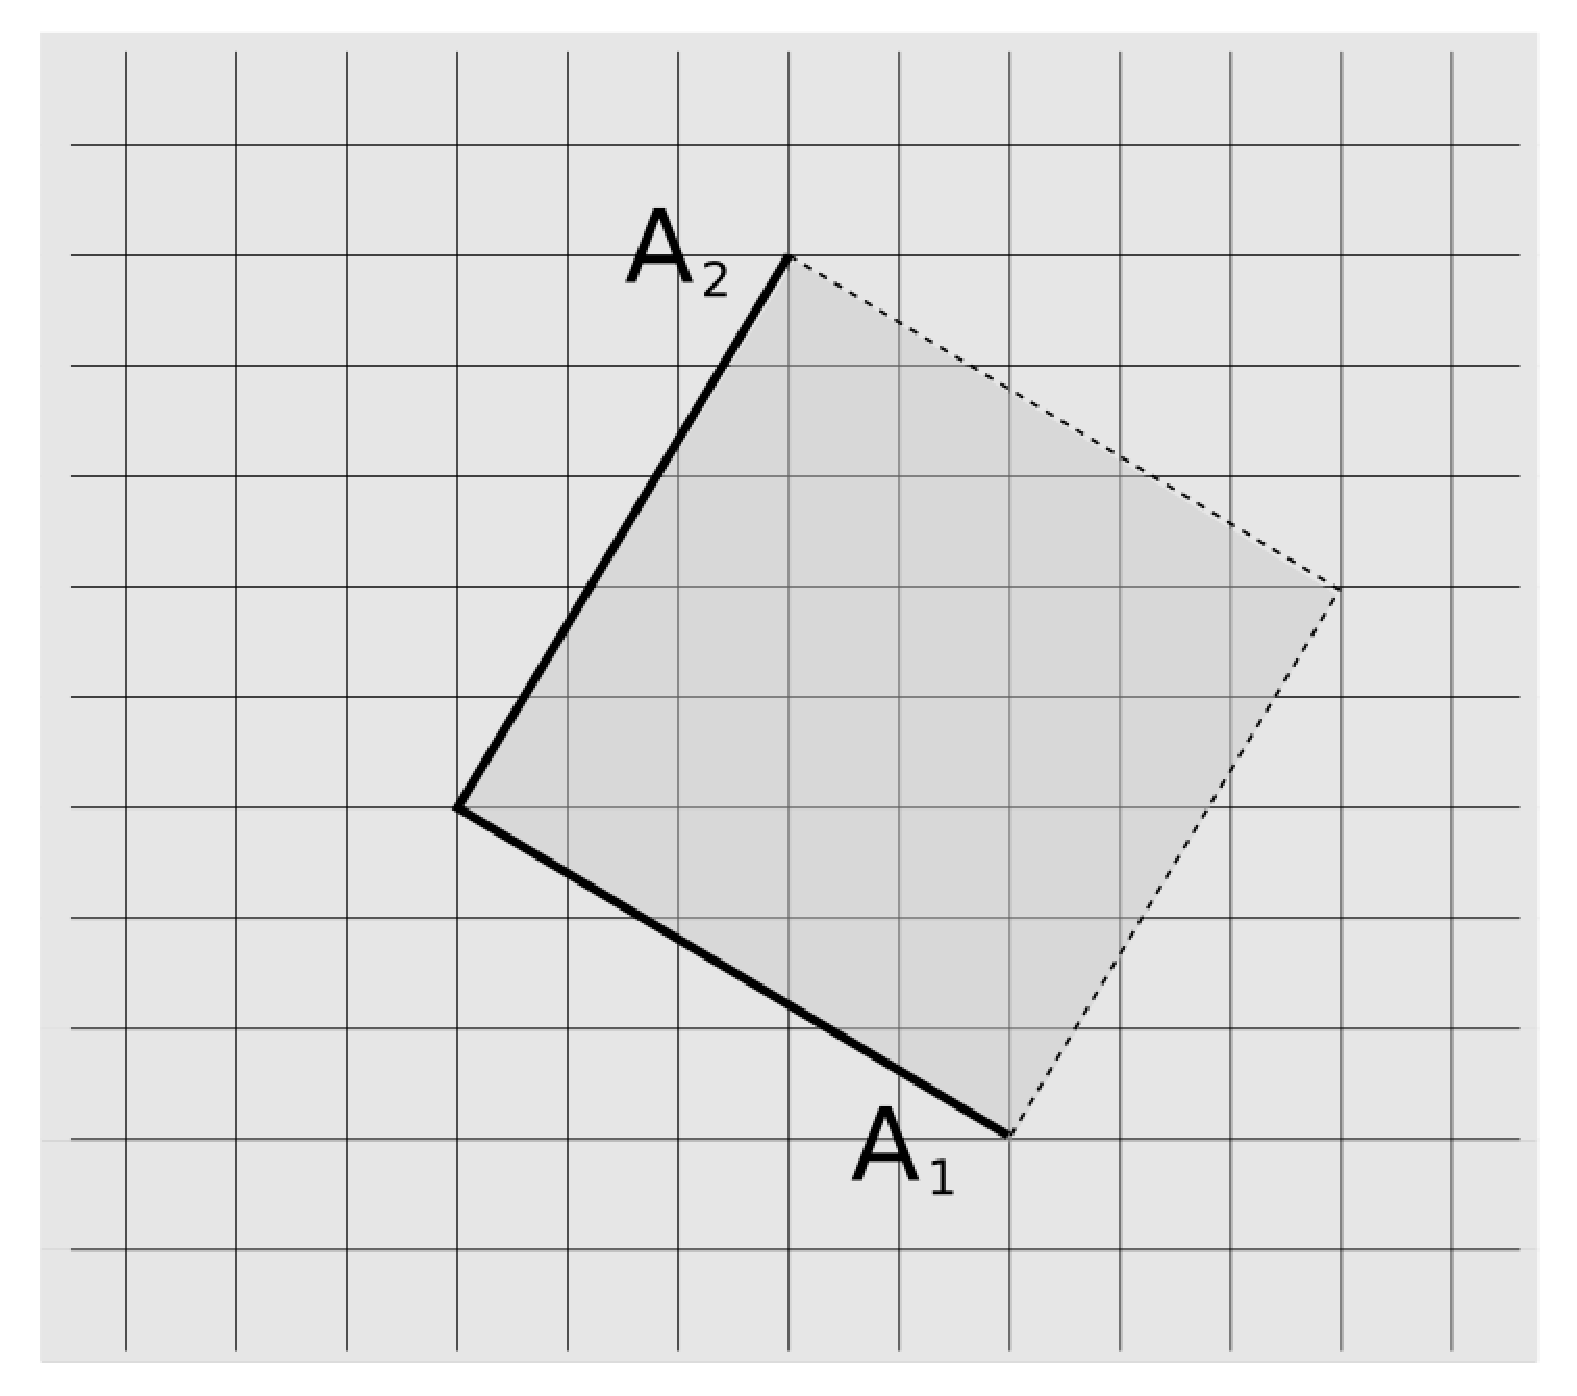
\includegraphics{figures/pythagoras.pdf}}
\caption{}
\end{figure}


\begin{figure}[H]
\label{fig:Bezout}
\scalebox{.3}{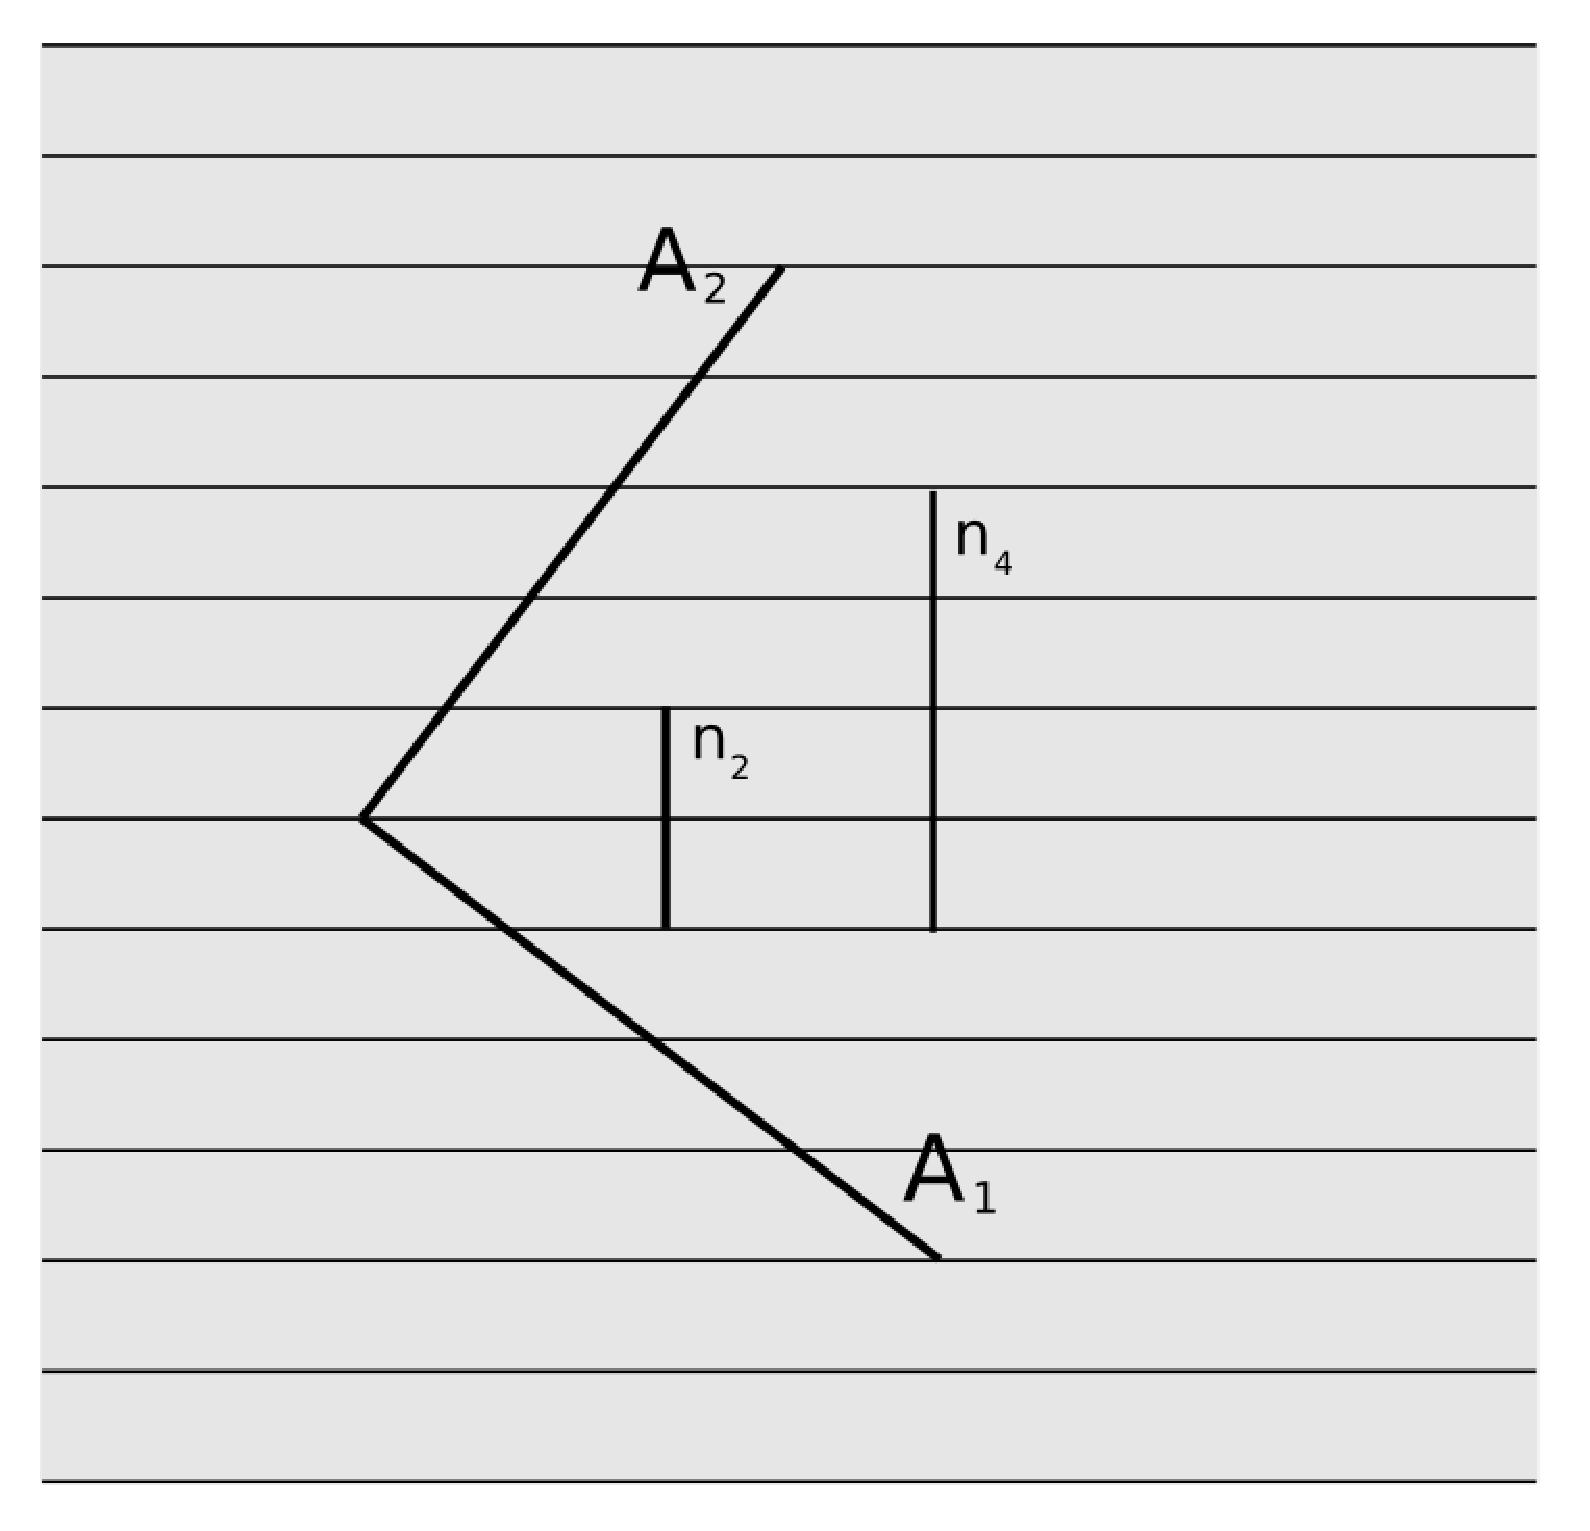
\includegraphics{figures/Bezout.pdf}}
\caption{}
\end{figure}
